%%jslbeamer

% \documentclass[handout, aspectratio=169]{beamer}
\documentclass[aspectratio=169]{beamer}
\setlength{\parskip}{.8em}

\definecolor{baseline-gray}{HTML}{f0f2f2}
\definecolor{baseline-red}{HTML}{ff5043}
\definecolor{baseline-blue}{HTML}{2d3bff}
\definecolor{b-violet}{HTML}{7d37bf}
% \definecolor{b-green}{HTML}{0BB350}
\definecolor{b-green}{HTML}{33c664}
\definecolor{b-yellow}{HTML}{f4e511}

\colorlet{couleurFond}{baseline-gray}
\colorlet{couleurTheme}{baseline-blue}
\colorlet{couleurSecondaire}{baseline-red}

\usepackage{myBeamer}
\usepackage{graphbox}
\usepackage{ragged2e}
% \usepackage{tabularx}
\usepackage{booktabs}

\usetikzlibrary{positioning}


\title{Communiquer efficacement ses données: un guide pratique}
\author[J.S. Leboeuf]{Jean-Samuel Leboeuf}
\date{5 mai 2021}


\tikzset{
  fleche/.tip={>[length=5pt,width=8pt]},
  rarr/.style={-fleche, line width=.8pt, line cap=rect},
  larr/.style={fleche-, line width=.8pt, line cap=rect},
  lrarr/.style={fleche-fleche, line width=.8pt, line cap=rect}
}

\tikzset{
  inline/.style={baseline=-1.25ex,
  				 every node/.style={inner sep=0pt, outer sep=0pt}
  				}
}

\tikzset{
	>={To[scale=1.1]},
	every picture/.style={->,thick},
}




\begin{document}


\begin{frame}
\thispagestyle{empty}
\titlepage
\end{frame}

% Être capable de partager efficacement ses résultats est une part importante de la communication scientifique. Cet exposé se veut un guide pratique sur le choix du moyen de communication des données (ex.: tableaux, diagrammes à courbes, diagrammes à bandes, etc.) ainsi que sur la manière de les présenter efficacement et professionnellement.

% Guide pratique sur la communication efficace des données à l'aide de tableaux et de figures.
%




% Intro:
% On vous a montré comment écrire un essai/rapport: intro, hypothèses/position, méthodologie et résultats/arguments, analyse, conclusion.

% On ne vous a pas enseigné comment présenter vos résultats de manière convaincante: le prof connaît l'expérience, sait à quoi s'attendre, sait quelle variable doit être mesurée et utilisée pour valider l'hypothèse. Il n'a pas à comprendre ce que vous faites: il sait si vous avez bien fait ou non.

% C'est différent de la vraie recherche: vous devez inventer l'expérience, choisir les variables à mesurer, et présenter l'expérience de manière claire pour faire comprendre et pour convaincre la communauté scientifique.

% Cette présentation vise à donner des pistes pour communiquer plus clairement et plus efficacement vos recherches en appliquant le "principe de correction négative". Plus spécifiquement, je donnerai des trucs pour mieux présenter vos données avec des exemples concrets en LaTeX.


\begin{frame}[t]\frametitle{La communication scientifique}

\vspace{3mm}
\begin{tikzpicture}[remember picture, overlay, shift=(current page.center)]
\node at (0,0) {
  \begin{tikzpicture}[inner sep=0pt, outer sep=2mm]
	\node[font=\small](intro) {Intro\vphantom{qM}};
	\node[font=\small, right=0mm of intro](prob) {Problématique\vphantom{qM}};
	\node[font=\small, right=0mm of prob](hyp) {Hypothèse\vphantom{qM}};
	\node[font=\small, right=0mm of hyp](metho) {Méthodologie\vphantom{qM}};
	\node[font=\small, right=0mm of metho](result) {Résultats et analyse\vphantom{qM}};
	% \node[font=\small, right=0mm of result](analyse) {Analyse\vphantom{qM}};
	\node[font=\small, right=0mm of result](conclu) {Conclusion\vphantom{qM}};

	\visible<2->{
	\node[couleurTheme, above=8mm of prob](donne prob) {Donnée};
	\node[couleurTheme, above=8mm of metho](donne metho) {Donnée};
	\draw[couleurTheme, ->] (donne prob) -- (prob);
	\draw[couleurTheme, ->] (donne metho) -- (metho);
	\draw[couleurTheme, ->] (metho) edge[bend left=45] (result);
	}

	\visible<3->{
	\node[couleurSecondaire, below=8mm of prob](trouver prob) {À trouver};
	\draw[couleurSecondaire, ->] (trouver prob) -- (prob);
	\draw[couleurSecondaire, <-] (result) edge[bend left=65] (hyp);
	\draw[couleurSecondaire, ->] (result) edge[bend left=45] (metho);
	}
  \end{tikzpicture}
};
\end{tikzpicture}

\vspace{35mm}

% Ce qui est différent:
\begin{itemize}
	\item<4-> Les résultats doivent être \textbf{convaincants} et \textbf{faciles à comprendre}
	% \item La méthodologie doit être \textbf{justifiée}
\end{itemize}
% Les résultats doivent être \textbf{facile à comprendre} et être \textbf{convaincants}

\end{frame}



\begin{frame}[c]\frametitle{Communication efficace}
\onslide<+->
Pour être \textbf{convaincants}, il faut:\vspace{-\parskip}
\begin{itemize}
	\item Des données pertinentes à l'hypothèse
\end{itemize}

Pour être \textbf{faciles à comprendre}, il faut:\vspace{-\parskip}
\begin{itemize}
	\item Éviter les données ambigües
	\item Éviter les éléments superflus
\end{itemize}

\onslide<+->
On peut appliquer le principe de \og coût initial négatif \fg


\end{frame}


\begin{frame}[c]\frametitle{Plan}
    
\tableofcontents

\end{frame}


\section{Le principe de coût initial négatif}
\label{sec:le_principe_de_coût_initial_négatif}



\begin{frame}[c]\frametitle{Coût initial négatif}
    
    
\vspace{-5mm}
\centering
\begin{tikzpicture}
\draw[->] (-5,0) -- (5,0) node[pos=1, anchor=west, align=left] {Valeur\\ intrinsèque};
\visible<2>{
\draw[->] (0,-2) -- (0,2) node[pos=1, anchor=south, align=left] {Valeur\\ ajoutée};
}

\fill[opacity=.2, couleurTheme] (0, 0) ellipse [x radius=1cm, y radius=.7cm];
\fill[opacity=.2, couleurSecondaire] (-3, 0) ellipse [x radius=1.8cm, y radius=.7cm];
\fill[opacity=.2, b-green] (2.8, 0) ellipse [x radius=1.6cm, y radius=.7cm];

\visible<1>{
\node[couleurSecondaire] at (-3.5, 1.3) {Faux, ambigü, contradictoire};
\node[couleurTheme] at (0, -1.3) {Superflu, redondant, distrayant};
\node[b-green] at (4, 1.3) {Utile, convaincant};
\draw[->] (-5,0) -- (5,0) node[pos=1, anchor=west, align=left] {Valeur\\ intrinsèque};
\draw[-] (0,.2) -- (0,-.2) node[below] {0};
}

\visible<2>{
\draw[-, couleurTheme] (-2,-1.8) -- (4.2,1.8);
\node[anchor=west](cout) at (.6, -1.1) {Coût initial négatif};
\draw (cout.west) to[out=180, in=-35] (.05,-.8);
}




\end{tikzpicture}

\end{frame}



\begin{frame}[c]\frametitle{Présentation des résultats}

\centering    
\begin{tikzpicture}

\node(exp) at (0, 1.2) {Expérience\vphantom{Mg}};
\node(donnees) {Données\vphantom{Mg}};
\node(tab) at (-2.9,-1.7) {\bf Tableaux\vphantom{Mg}};
\node<1>(graph) at (2.9,-1.7) {\bf Graphiques\vphantom{Mg}};
\node<2>[opacity=.5] at (2.9,-1.7) {\bf Graphiques\vphantom{Mg}};

\draw (exp) -- (donnees);
\draw (donnees) edge[out=-90, in=90] (tab);
\draw (donnees) edge[out=-90, in=90] (graph);

\node[below=0mm of tab] {
\begin{minipage}{.48\textwidth}
\begin{itemize}
	\item Condensé de données disparates
	\item Comparaisons quantitatives
	\item Valeurs exactes
\end{itemize}
\end{minipage}
};

\node<1>[below=0mm of graph] {
\begin{minipage}{.43\textwidth}
\begin{itemize}
	\item Visualisation des données
	\item Comparaison qualitative
	\item Extraction de tendances
\end{itemize}
\end{minipage}
};
\node<2>[below=0mm of graph, opacity=.5] {
\begin{minipage}{.43\textwidth}
\begin{itemize}
	\item Visualisation des données
	\item Comparaison qualitative
	\item Extraction de tendances
\end{itemize}
\end{minipage}
};

\end{tikzpicture}

\end{frame}





\section{Les tableaux}
\label{sec:les_tableaux}





\begin{frame}[c]\frametitle{Deux types de tableaux}

\vspace{-3mm}

\begin{tabular}{@{}ll@{}}
Tableau de \textbf{communication} & Tableau de \textbf{compilation}\\
\begin{minipage}[t]{.52\textwidth}
\begin{itemize}
	\item<2-> Résumé utile des informations
	\item<2-> Concis et facile à lire
	\item<2-> Ne contient pas toutes les informations (coût initial négatif)
	\item<2-> Met en évidence des différences ponctuelles
	\item<2-> Dans le \textbf{corps} d'un document
\end{itemize}
\end{minipage}
& 
\begin{minipage}[t]{.48\textwidth}
\begin{itemize}
	\item<3-> Contient toutes les informations recueillies
	\item<3-> Se veut une référence
	\item<3-> Longs et plates à lire
	\item<3-> Dans l'\textbf{annexe} d'un document
\end{itemize}
\end{minipage}
\end{tabular}


\end{frame}


\begin{frame}[c]\frametitle{Les tableaux de communication}

% \begin{tabular}{ll}
% \bf Pros & \bf Cons \\[5pt]
% \begin{minipage}{.35\textwidth}
% \begin{itemize}
% 	\item Dense et compact
% 	\item Précis
% \end{itemize}
% \end{minipage}
% &
% \begin{minipage}{.6\textwidth}
% \begin{itemize}
% 	\item Difficile d'extraire des tendances
% 	\item Peu visuel
% \end{itemize}
% \end{minipage}
% \end{tabular}


% \begin{tabular}{||c|c|c||}
% \hline
% \multirow{2}{*}{Boeuf} & kg & 13,65\$ \\
% \cline{2-3}
%  & lbs & 7,99 \\ 
% \hline
% Poulet & \multirow{2}{*}{Farci} & 5,99 \\ 
% \cline{1-1}
% \cline{3-3}
% Dinde &  & 10,99 \\ 
% \hline
% Porc & Congelé & 4,99\\
% \hline
% \end{tabular}


\begin{tabular}{p{.5\textwidth}c}
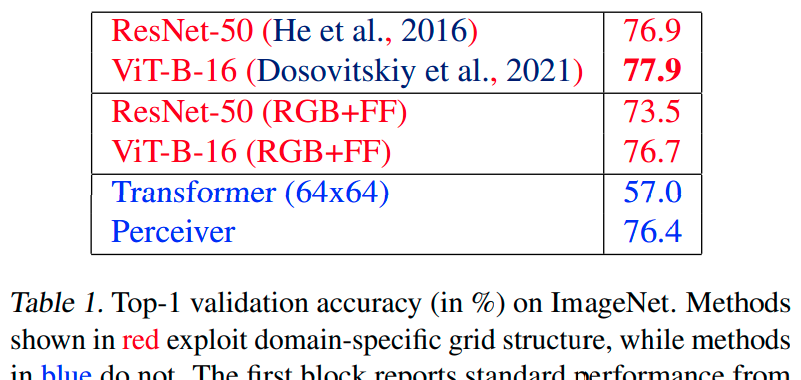
\includegraphics[width=.5\textwidth]{figures/bad-table.png}\\
\scriptsize\raggedright
Tiré de l'article «~Perceiver: General Perception with Iterative Attention~» par DeepMind (Google)
&
\visible<2->{
\begin{minipage}{.4\textwidth}
\vspace{-3.5cm}
\begin{table}\rmfamily\scriptsize\RaggedRight
Table~1.\ Top\hspace{1pt}-\hspace{-1.08pt}1 validation accuracy on ImageNet. Blablabla\dots

\vspace{3pt}
\begin{tabular}{l@{\hskip5pt}r@{\hskip10pt}r@{\hskip5pt}c}
\toprule
\multirow{2}{*}[-2pt]{Model} & \multicolumn{2}{c}{Top\hspace{1pt}-\hspace{-1.08pt}1 (\%)} & \multirow{2}{*}[-2pt]{Uses grid}\\
\cmidrule(r){2-3}
 & No FF & FF & \\
\midrule
ResNet-50 & 76.9 & 73.5 & yes\\
ViT-B-16 & \textbf{77.9} & 76.7 & yes\\
Transformer & --- & 57.0 & no\\
Perceiver & --- & 76.4 & no\\
\bottomrule
\end{tabular}
\end{table}
\end{minipage}
}

\end{tabular}



\end{frame}


\begin{frame}[c]\frametitle{Conseils généraux}

\vspace{-4mm}

\begin{itemize}
	\item<+-> Tableau $\ne$ grille:
	\begin{itemize}
		\item Lignes horizontales: début, fin et entre les sections seulement
		\item JAMAIS de lignes verticales: ajuster l'espace entre les colonnes
	\end{itemize}
	\vspace{-3mm}
	\item<+-> Étiquettes des colonnes avec unités et abbréviations limitées
	\item<+-> Titre \textit{au-dessus} du tableau avec explications
	\item<+-> Éviter les répétitions
	\item<+-> Citer dans le titre ou le texte
	\item<+-> Mettre en évidence une seule chose à la fois
	\item<+-> Éviter les couleurs
	\item<+-> Référer au tableau explicitement dans le texte
	\item<+-> Aligner les chiffres à droite, le texte à gauche
\end{itemize}

\end{frame}


\begin{frame}[fragile]\frametitle{Tableaux professionnels avec LaTeX}

\vspace{-3mm}

Les packages:
\vspace{-\parskip}
\begin{itemize}
	\item \texttt{booktabs}: Redéfinit entièrement les tableaux (\href{https://ctan.mirror.rafal.ca/info/translations/booktabs/fr/f-booktabs.pdf}{\underline{documentation}})
	\item \texttt{multicol} et \texttt{multirow}: Fusionner des cellules
\end{itemize}

Les lignes:
\vspace{-\parskip}
\begin{itemize}
	\item \verb!\toprule! et \verb!\bottomrule! pour les lignes du haut et du bas
	\item \verb!\midrule! pour les lignes entre sections
	\item \verb!\cmidrule(lr){<col début>-<col fin>}! pour les lignes partielles
\end{itemize}

Les cellules fusionnées:
\vspace{-\parskip}
\begin{itemize}
	\item \verb!\multirow{<n rangées>}{*}[<y shift>]{<contenu>}! pour les rangées
	\item \verb!\multicolumn{<n col>}{c}{<contenu>}! pour les colonnes
\end{itemize}

\end{frame}


\begin{frame}[fragile]\frametitle{Tableaux professionnels avec LaTeX}

\vspace{-3mm}

Les colonnes:
\vspace{-\parskip}
\begin{itemize}
	\item \verb!@{\hskip<distance>}! pour ajuster la distance entre deux colonnes
\end{itemize}

Le titre:
\vspace{-\parskip}
\begin{itemize}
	\item \verb!\caption{<titre>}! pour le titre
	\item \verb!\vspace{<distance>}! pour ajuster la distance entre le titre et le tableau
\end{itemize}

Outil d'aide à la génération de tableaux:
\vspace{-\parskip}
\begin{itemize}
	\item \url{https://www.tablesgenerator.com/}
	\item \href{https://github.com/jsleb333/python2latex}{\underline{python2latex}} (Création du code LaTeX à partir de \texttt{numpy arrays})
\end{itemize}


\end{frame}









\begin{frame}[fragile]\frametitle{Exemple}
\vspace{-7mm}

\begin{tabular}{ll}
\tiny
\begin{minipage}{.55\textwidth}
\begin{verbatim}
\usepackage{booktabs}

\begin{table}
\caption{Top-1 validation accuracy on ImageNet.}
\label{tab:top1_imagenet}
\vspace{3pt}
\begin{tabular}{l@{\hskip5pt}r@{\hskip10pt}r@{\hskip5pt}c}
\toprule
\multirow{2}{*}[-2pt]{Model}
    & \multicolumn{2}{c}{Top-1 (\%)}
    & \multirow{2}{*}[-2pt]{Uses grid}\\
\cmidrule(r){2-3}
 & No FF & FF & \\
\midrule
ResNet-50   & 76.9 & 73.5 & yes\\
ViT-B-16    & \textbf{77.9} & 76.7 & yes\\
Transformer & --- & 57.0 & no\\
Perceiver   & --- & 76.4 & no\\
\bottomrule
\end{tabular}
\end{table}
\end{verbatim}
\end{minipage}
& 
\begin{minipage}{.39\textwidth}
\scriptsize\rmfamily
Top-1 validation accuracy on ImageNet.
\vspace{6pt}
\begin{tabular}{l@{\hskip5pt}r@{\hskip10pt}r@{\hskip5pt}c}
\toprule
\multirow{2}{*}[-2pt]{Model}
    & \multicolumn{2}{c}{Top-1 (\%)}
    & \multirow{2}{*}[-2pt]{Uses grid}\\
\cmidrule(r){2-3}
 & No FF & FF & \\
\midrule
ResNet-50   & 76.9 & 73.5 & yes\\
ViT-B-16    & \textbf{77.9} & 76.7 & yes\\
Transformer & --- & 57.0 & no\\
Perceiver   & --- & 76.4 & no\\
\bottomrule
\end{tabular}

\end{minipage}
\end{tabular}

\end{frame}




















\section{Principes premiers des figures}
\label{sec:principes_premiers_des_figures}



\begin{frame}[c]\frametitle{Les graphiques}

\centering    
\begin{tikzpicture}

\node(exp) at (0, 1.2) {Expérience\vphantom{Mg}};
\node(donnees) {Données\vphantom{Mg}};
\node[opacity=.5](tab) at (-2.9,-1.7) {\bf Tableaux\vphantom{Mg}};
\node(graph) at (2.9,-1.7) {\bf Graphiques\vphantom{Mg}};

\draw (exp) -- (donnees);
\draw (donnees) edge[out=-90, in=90] (tab);
\draw (donnees) edge[out=-90, in=90] (graph);

\node[below=0mm of tab, opacity=.5] {
\begin{minipage}{.48\textwidth}
\begin{itemize}
	\item Condensé de données disparates
	\item Comparaisons quantitatives
	\item Valeurs exactes
\end{itemize}
\end{minipage}
};

\node[below=0mm of graph] {
\begin{minipage}{.43\textwidth}
\begin{itemize}
	\item Visualisation des données
	\item Comparaison qualitative
	\item Extraction de tendances
\end{itemize}
\end{minipage}
};

\end{tikzpicture}


\end{frame}






\begin{frame}[c]
    
\vspace{-1pt}
\centering
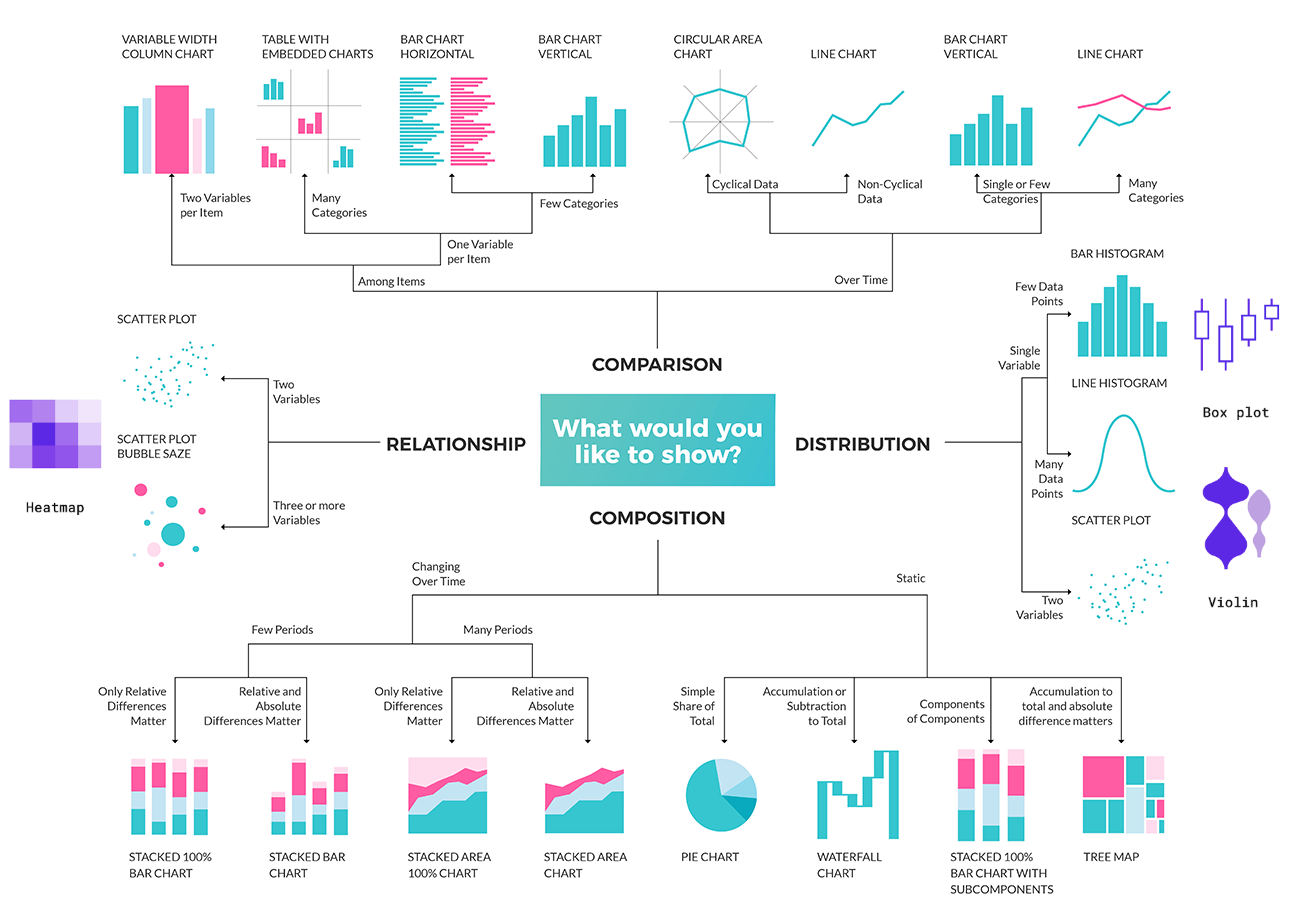
\includegraphics[height=\paperheight]{figures/types_of_charts.png}


\end{frame}




% \begin{frame}[c]\frametitle{Les types de graphiques}
    


% \textbf{Types} de graphiques:

% \begin{tabular}{l@{}l}
% \begin{minipage}{.45\textwidth}
% \begin{itemize}
% 	\item Courbes (\textit{line plot})
% 	\item Histogrammes (\textit{bar chart})
% 	\item Circulaires (\textit{pie chart})
% 	\item etc.
% \end{itemize}
% \end{minipage}
% &
% \begin{minipage}{.5\textwidth}
% \begin{itemize}
% 	\item Violons (\textit{violin plot})
% 	\item Boîtes à moustaches (\textit{box plot})
% 	\item Nuages de points (\textit{scatter plot})
% 	\item[]
% \end{itemize}
% \end{minipage}
% \end{tabular}


% \textbf{Trois situations} fréquentes:
% \vspace{-.8\parskip}
% \begin{enumerate}
% 	\item Comparer des séquences
% 	\item Visualiser des distributions
% 	\item Étudier des relations
% \end{enumerate}


% \end{frame}



\begin{frame}[c]\frametitle{Principes premiers d'une figure}

\begin{enumerate}\setlength\itemsep{2em}
	\item Représentation fidèle, non-trompeuse et sans distorsions

	\item Représentation claire et évidente

	\item Représentation facile à analyser et à comparer
\end{enumerate}

\end{frame}



\begin{frame}[c]\frametitle{Représentation fidèle}
    

\begin{itemize}
	\item Ne donne pas de fausses impressions
\end{itemize}

\begin{center}
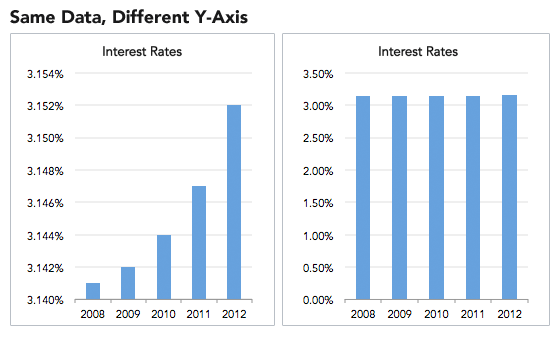
\includegraphics[width=.4\textwidth]{figures/misleading_chart.png}
\hspace{1cm}
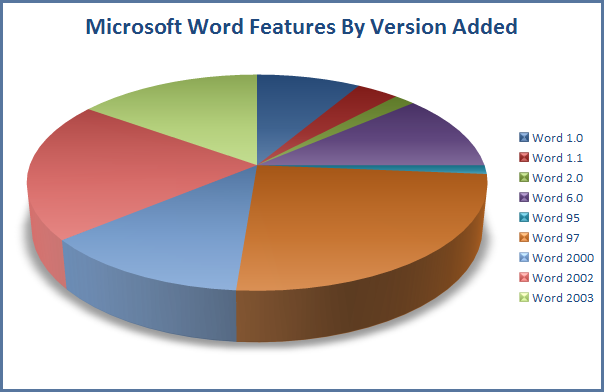
\includegraphics[width=.4\textwidth]{figures/misleading-pie-chart.png}
\end{center}

\end{frame}





\begin{frame}[c]\frametitle{Représentation claire}
    
% \begin{itemize}
% 	\item Auto-évidente, simple et facile à comprendre
% \end{itemize}
\begin{center}
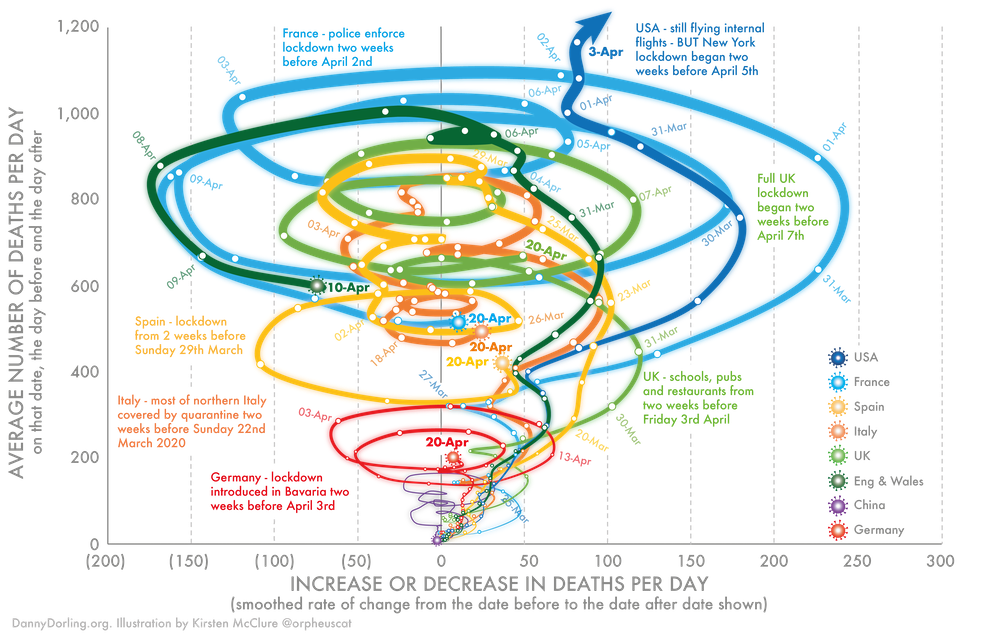
\includegraphics[scale=.25]{figures/unclear-chart.png} 
\end{center}

\end{frame}




\begin{frame}[c]\frametitle{Représentation facile à analyser}
    
\vspace{-3mm}

\centering
\onslide<+->
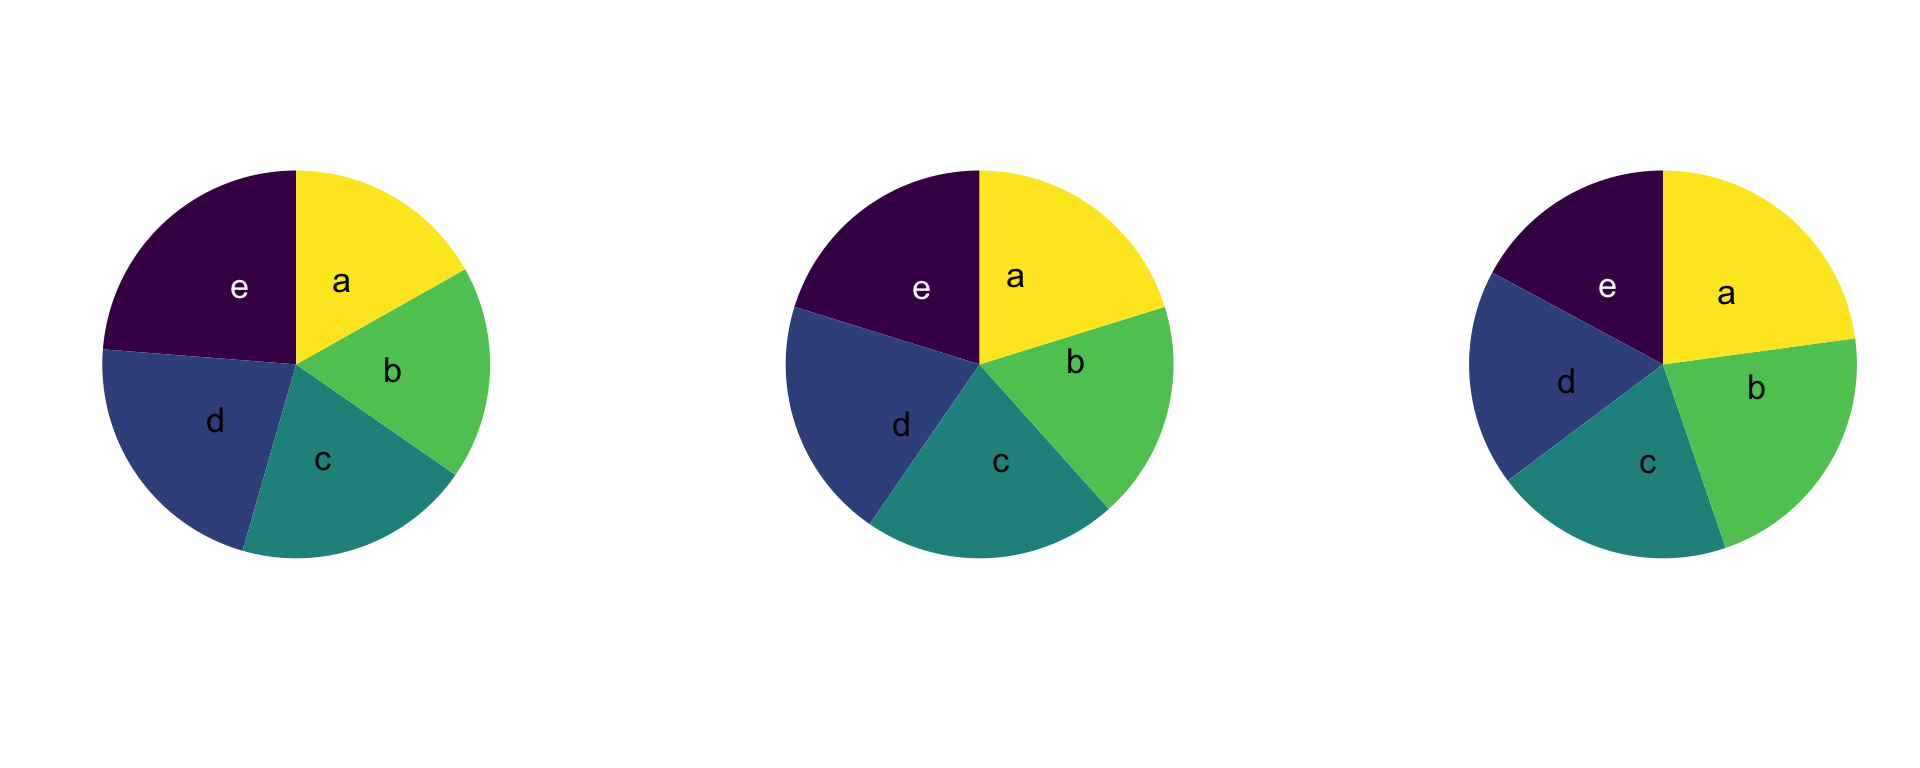
\includegraphics[width=.6\textwidth, trim={2cm 6.2cm 1cm 5cm}, clip]{figures/pie-charts-bad.png}
\onslide<+->
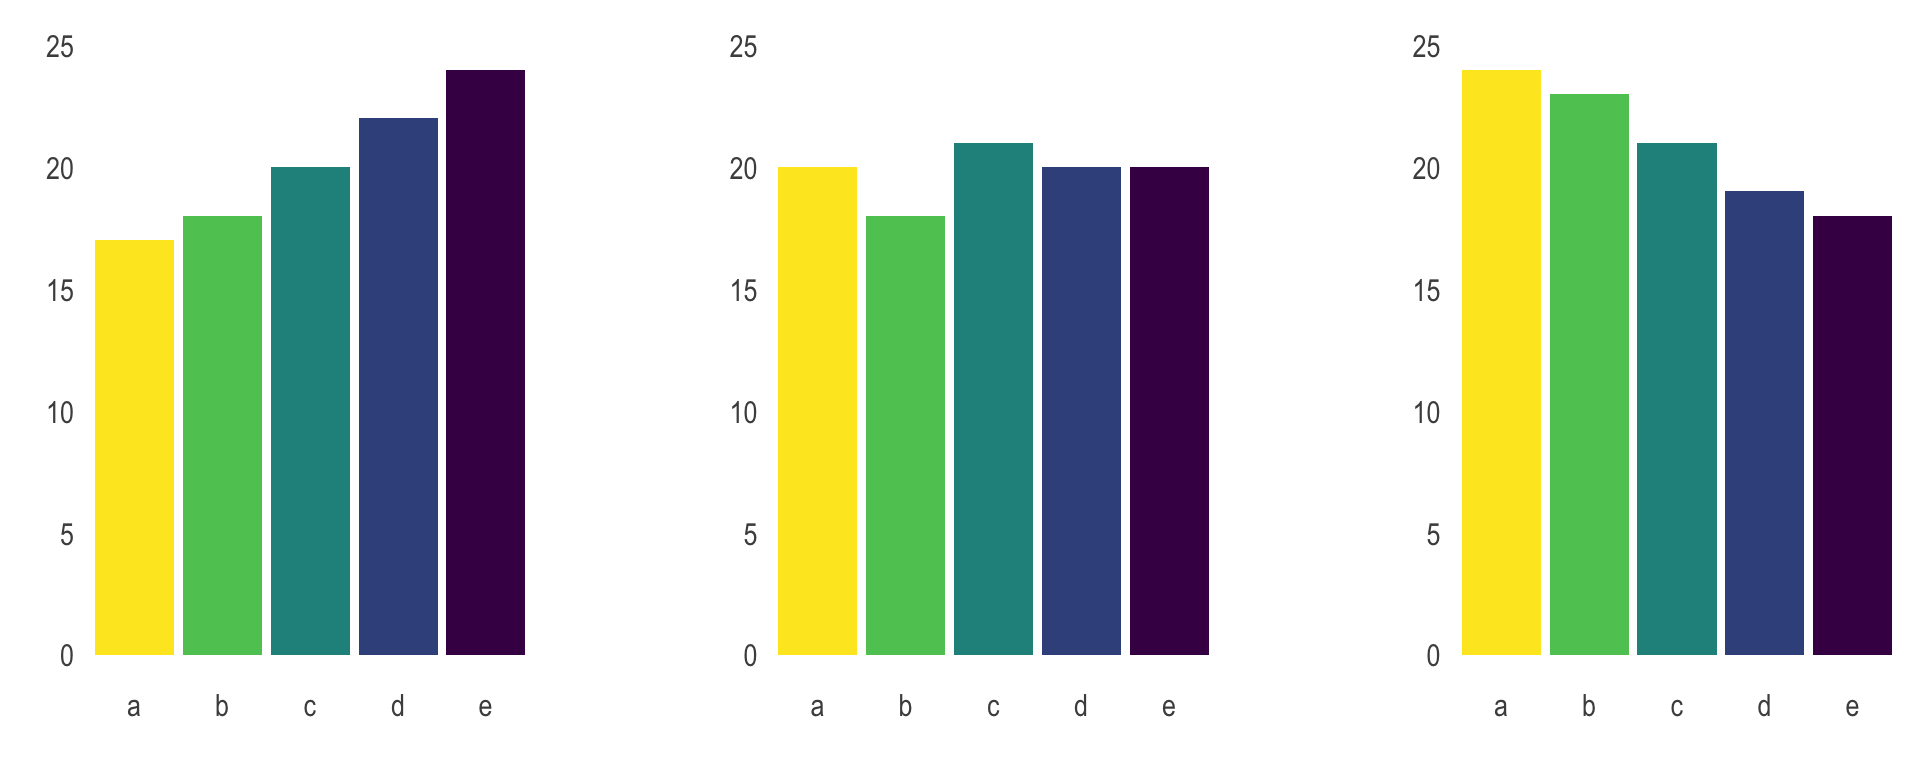
\includegraphics[width=.6\textwidth]{figures/bar-charts-good.png}

\begin{itemize}
	\item<4-> Le cerveau est poche pour comparer des aires et des distances
	\item<4-> Le cerveau est bon pour comparer des positions
\end{itemize}

\end{frame}



\begin{frame}[c]
    
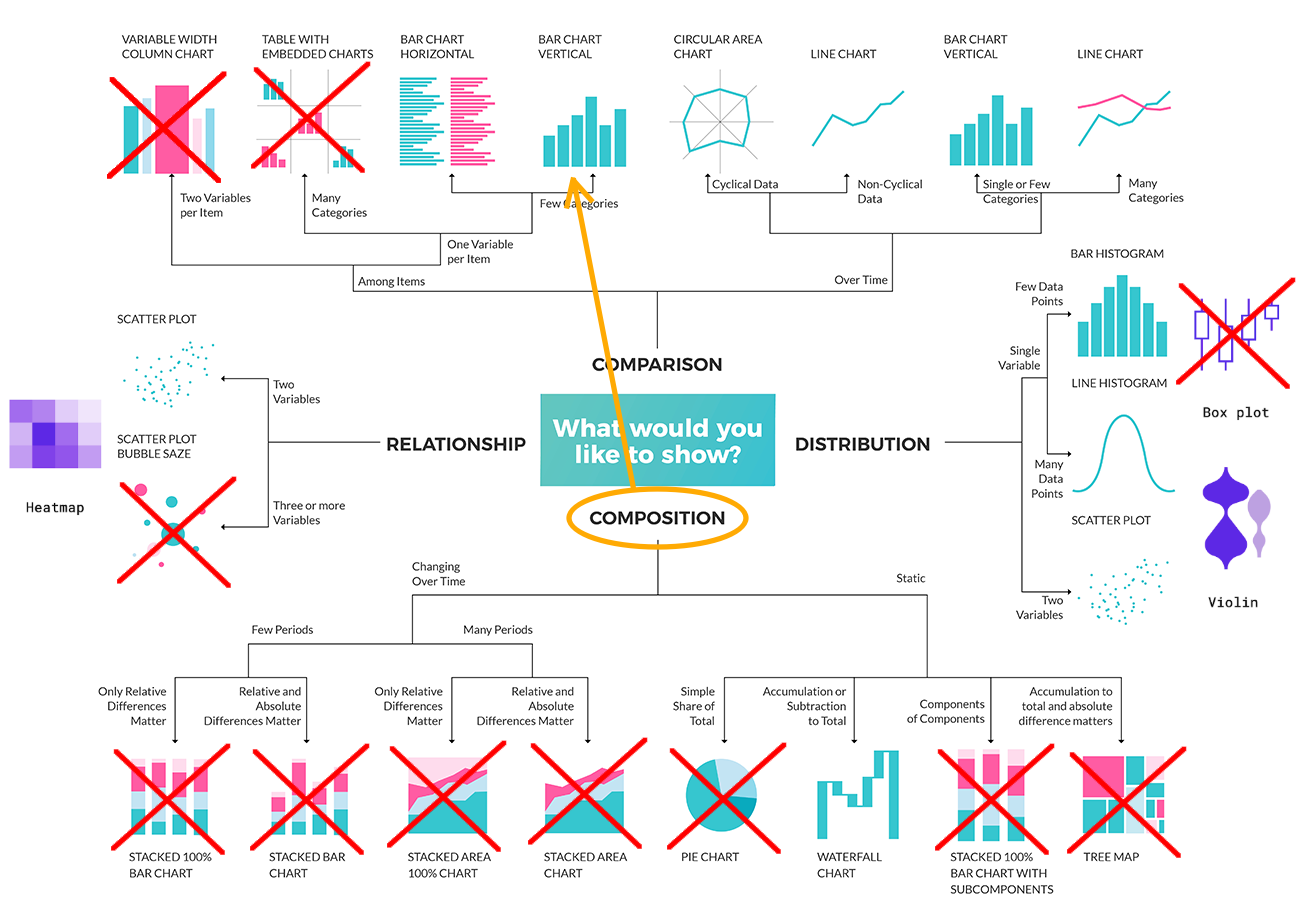
\includegraphics[height=\paperheight]{figures/types_of_charts_sorted.png}

\end{frame}






\section{Les types de graphiques}
\label{sec:les_types_de_graphiques}


\begin{frame}[c]\frametitle{Guide général de style}

Les \textbf{axes}:
\vspace{-\parskip}
\begin{itemize}
	\item En bas et à gauche seulement
	\item Étiquettes avec unité
	\item Discrétisation modérée (5 à 10)
	\item Police de taille similaire au texte
	\item Grille aérée et pâle; \textbf{pas} de fond
\end{itemize}

Le \textbf{titre}:
\vspace{-\parskip}
\begin{itemize}
	\item Préférablement sous la figure
	\item Numérotée et référencée dans le texte
	\item Explications spécifiques non redondantes
\end{itemize}

\end{frame}




\begin{frame}[c]\frametitle{Guide pour les courbes}

\begin{tabular}{@{}ll}
\begin{minipage}{.49\textwidth}
\begin{itemize}
	\item Éviter les légendes si possibles
	\begin{itemize}
		\item Sinon, lister les entrées en ordre d'apparition
	\end{itemize}
	\vspace{-3mm}
	\item Couleurs pour différencier les courbes
	\item Lignes pleines, discontinues ou pointillées pour différencier les familles de courbes
	\item 8 courbes maximum par diagrammes
\end{itemize}
\end{minipage}
& 
\colorbox{white}{
\begin{minipage}{.45\textwidth}
\begin{center}
\hspace*{-5mm}
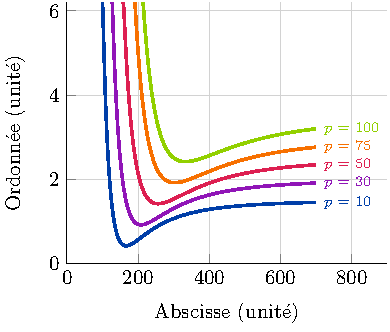
\includegraphics[width=.9\textwidth]{examples/lineplot_example.pdf}
\end{center}
\vspace{-5mm}
\scriptsize
\rmfamily
\hspace*{.01\textwidth}
\parbox{.95\textwidth}{\justify
Figure~1. Exemple d'un diagramme à courbes. La légende est remplacée par une étiquette placée à la fin des courbes, ce qui facilite la lecture du graphique.
}
\end{minipage}
}

\end{tabular}
\end{frame}



\begin{frame}[c]\frametitle{Guide pour les nuages de points}
    

\begin{tabular}{@{}ll}
\begin{minipage}{.49\textwidth}
\begin{itemize}
	\item Formes et couleurs pour distinguer les catégories
	\item Opacité pour les données superposées
	\item Pour une troisième variable: utiliser une carte de couleurs, pas la taille des points
\end{itemize}
\end{minipage}
& 
\colorbox{white}{
\begin{minipage}{.45\textwidth}
\begin{center}
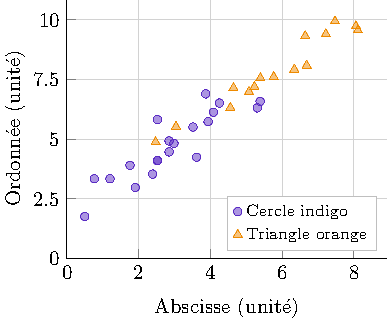
\includegraphics[width=.9\textwidth]{examples/scatterplot_example.pdf}
\end{center}
\vspace{-5mm}
\scriptsize
\rmfamily
\hspace*{.01\textwidth}
\parbox{.95\textwidth}{\justify
Figure~1. Exemple d'un nuage de point avec deux types de points. De la transparence est utilisée pour voir les points superposés.
}
\end{minipage}
}
\end{tabular}

\end{frame}



\begin{frame}[c]\frametitle{Guide pour les diagrammes à bandes}
    

\begin{tabular}{@{}ll}
\begin{minipage}{.49\textwidth}
\begin{itemize}
	\item Repères verticaux non-nécessaires
	\item Axe vertical commence à l'origine  
	\item Données près de la bande
	% \item Couleurs pour identifier des sous-catégories
	\item Bandes en ordre croissant
	\item Bandes à l'horizontal si les étiquettes ne rentrent pas (ne pas pivoter le texte)
\end{itemize}
\end{minipage}
& 
\colorbox{white}{
\begin{minipage}{.45\textwidth}
\begin{center}
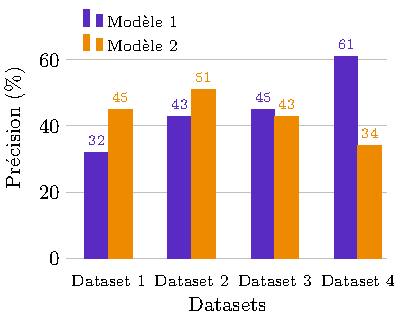
\includegraphics[width=.9\textwidth]{examples/bar_chart_example.pdf}
\end{center}
\vspace{-5mm}
\scriptsize
\rmfamily
\hspace*{.01\textwidth}
\parbox{.95\textwidth}{\justify 
Figure~1. Exemple d'un diagramme à bandes avec des catégories.
}
\end{minipage}
}
\end{tabular}

\end{frame}



\begin{frame}[c]\frametitle{Guide pour les «~heatmaps~»}
    
\begin{tabular}{@{}ll}
\begin{minipage}{.45\textwidth}
\begin{itemize}
	\item Se lit comme une matrice: origine en haut à droite
	\item Carte de couleurs:
	\begin{itemize}
		\item Séquentielle pour marquer l'intensité
		\item Divergente pour marquer la différence p/r à une valeur de référence
	\end{itemize}
	\vspace{-10pt}
	\item Blanc pour les données non pertinentes
	\item Annotations pour les données pertinentes
\end{itemize}
\end{minipage}
& 
\colorbox{white}{
\begin{minipage}{.5\textwidth}
\begin{center}
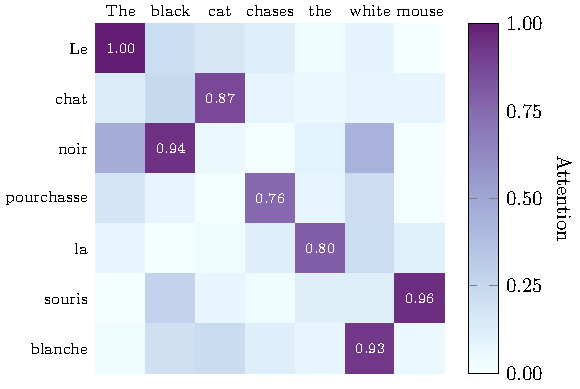
\includegraphics[width=\textwidth]{examples/heatmap_example.pdf}
\end{center}
\vspace{-5mm}
\scriptsize
\rmfamily
\hspace*{.01\textwidth}
\parbox{.95\textwidth}{\justify 
Figure~1. Exemple d'une «~heatmap~» pour l'attention d'un réseau pendant la traduction. Seuls les points d'intérêts sont annotés.
}
\end{minipage}
}
\end{tabular}

\end{frame}




\begin{frame}[c]\frametitle{Guide pour les violons}
    
\begin{tabular}{@{}ll}
\begin{minipage}{.49\textwidth}
\begin{itemize}
	\item «~Boîte à moustaches ++~»
	\item Permet d'identifier les modes
	\item Peuvent être groupés comme les diagrammes à bandes
	\item Normaliser l'\textbf{aire}, pas la largeur
\end{itemize}
\end{minipage}
& 
\colorbox{white}{
\begin{minipage}{.45\textwidth}
\begin{center}
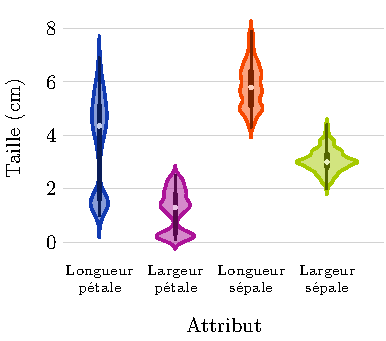
\includegraphics[width=.9\textwidth]{examples/violin_plot_example.pdf}
\end{center}
\vspace{-5mm}
\scriptsize
\rmfamily
\hspace*{.01\textwidth}
\parbox{.95\textwidth}{\justify 
Figure~1. Exemple d'un diagramme à violons pour la distribution des attributs du jeu de données \texttt{iris}. Les lignes intérieures correspondent à un \textit{box plot}.
}
\end{minipage}
}
\end{tabular}

\end{frame}


\begin{frame}[c]\frametitle{En résumé}
    
\begin{itemize}
	\item Favoriser les graphiques qui reposent sur le \textbf{positionnement}
	\item Ne pas surcharger le graphiques
	\item Annoter sur la figure plutôt qu'utiliser une légende
	\item Soyez constant dans le style entre les figures
\end{itemize}

\textbf{Références utiles}:\vspace{-\parskip}    
\begin{itemize}
	\item \href{https://material.io/design/communication/data-visualization.html}{\underline{Guide de visualisation de données de Material}}
\end{itemize}

\end{frame}



\begin{frame}[c]\frametitle{Outils}
    
\textbf{LaTeX:}\vspace{-\parskip}
\begin{itemize}
	\item Nativement avec les packages \href{https://ctan.mirror.colo-serv.net/graphics/pgf/base/doc/pgfmanual.pdf}{\underline{TikZ}} et \href{https://mirror.its.dal.ca/ctan/graphics/pgf/contrib/pgfplots/doc/pgfplots.pdf}{\underline{PGFPLOTS}}
	\item À partir de Python avec \href{https://github.com/jsleb333/python2latex}{\underline{python2latex}} ou \href{https://github.com/nschloe/tikzplotlib}{\underline{tikzplotlib}}
\end{itemize}

\textbf{Python}:\vspace{-\parskip}
\begin{itemize}
	\item \href{https://matplotlib.org/}{\underline{matplotlib}} avec \href{https://seaborn.pydata.org/index.html}{\underline{seaborn\vphantom{p}}}
	\vspace{1.5mm}
	\begin{itemize}
		\item PDF seulement, pas de PNG ou JPEG
		\item Attention à la taille du texte
		\item Les paramètres par défaut sont \textbf{mauvais}
	\end{itemize}
\end{itemize}

\end{frame}




\section{Les couleurs}
\label{sec:les_couleurs}


\begin{frame}[c]\frametitle{Les couleurs}

\vspace{-2mm}
% \textbf{Utilité:}\vspace{-\parskip}
\onslide<2->
\begin{minipage}[t]{.49\textwidth}
\centering
\textbf{Esthétique}
\vspace*{3mm}

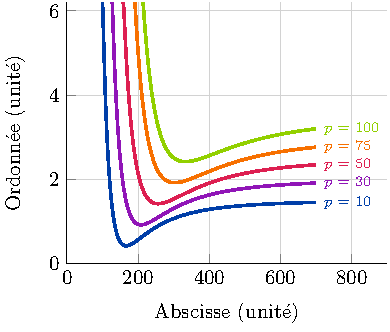
\includegraphics[scale=.45]{examples/lineplot_example.pdf}
\end{minipage}
\onslide<3->
\begin{minipage}[t]{.49\textwidth}
\centering
Différencier des \textbf{catégories}
\vspace*{3mm}

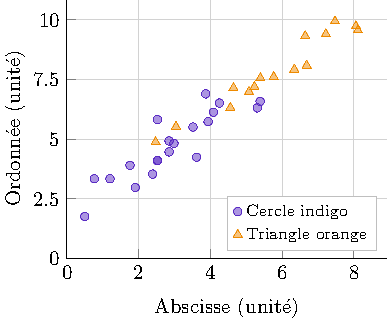
\includegraphics[scale=.45]{examples/scatterplot_example.pdf}
\end{minipage}


\onslide<4->
\begin{minipage}[t]{.49\textwidth}
\centering
Représenter un \textbf{spectre}
\vspace*{3mm}

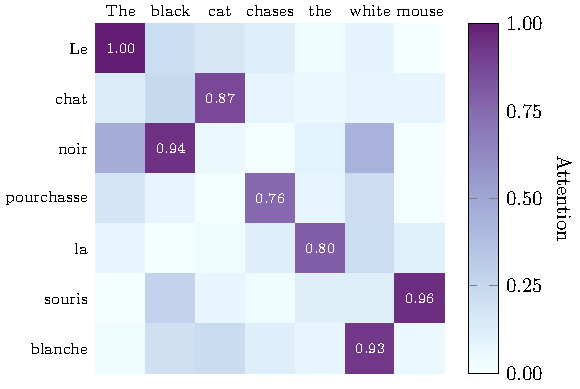
\includegraphics[scale=.35]{examples/heatmap_example.pdf}
\end{minipage}
\onslide<5->
\begin{minipage}[t]{.49\textwidth}
\centering
Mettre en \textbf{évidence}
\vspace*{3mm}

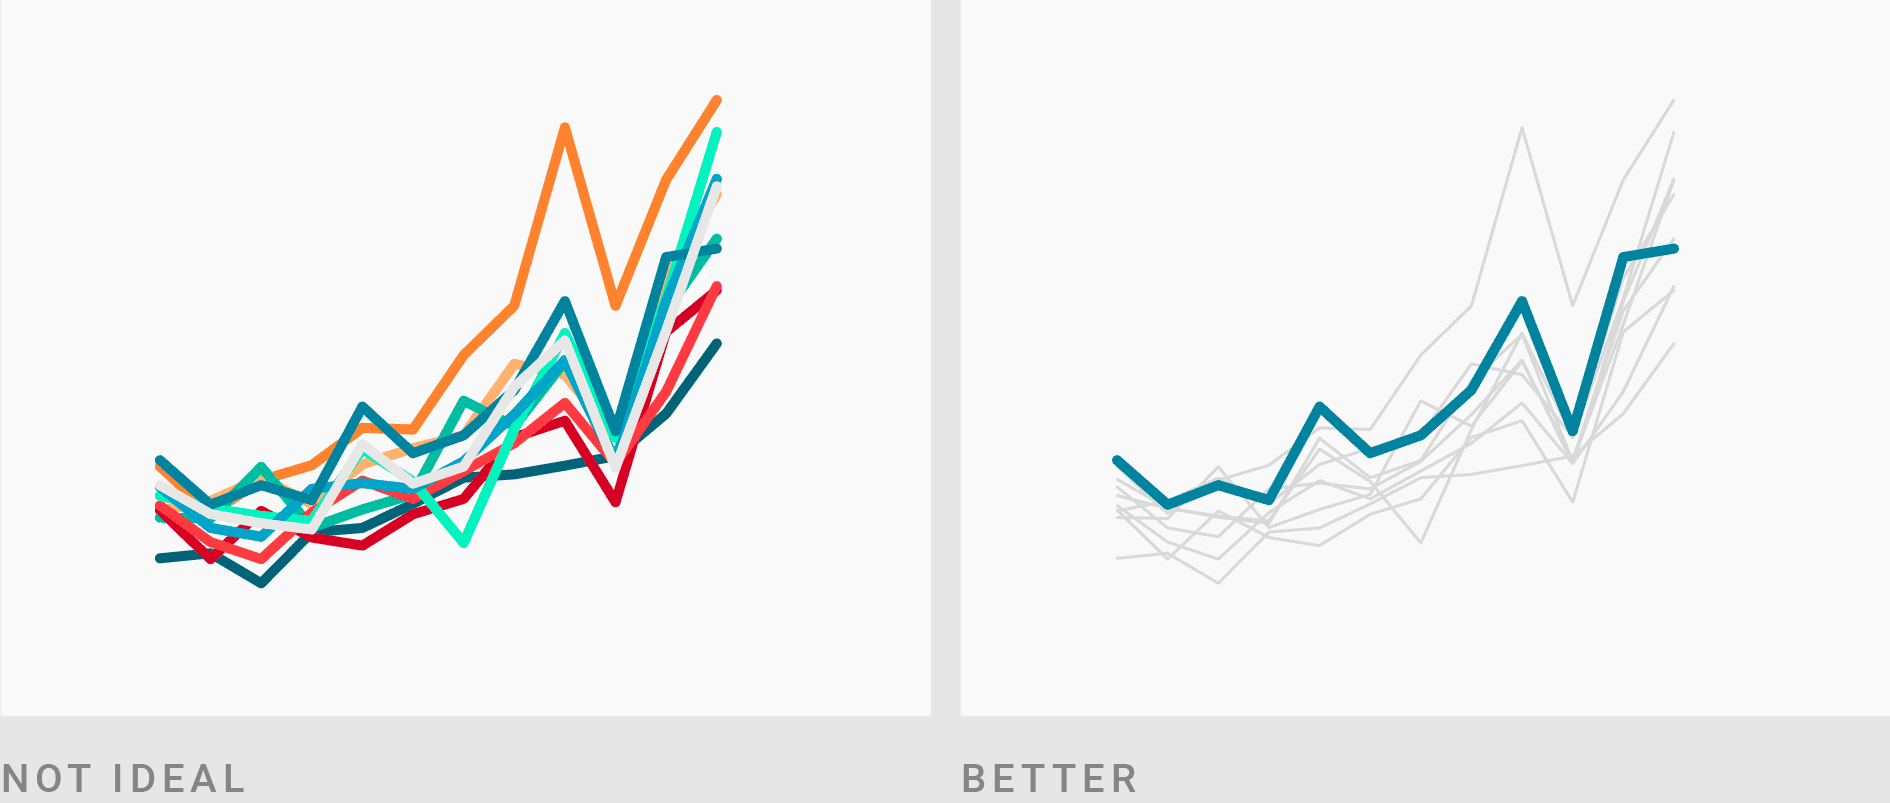
\includegraphics[width=.9\textwidth, trim={0 4cm 0 0}, clip]{figures/mise-en-evidence.png}
\end{minipage}
\end{frame}



\begin{frame}[t]\frametitle{Limitations}

% \vspace*{-4mm}


\begin{itemize}\setlength{\itemsep}{2pt}
	\item<1-> Difficile de comparer des couleurs semblables
	\item<2-> Perception affectée par les couleurs environnantes
	\item<4-> Les moniteurs et les imprimantes donnent des rendues différents
	\item<5-> Sort mal en tons de gris

	\item<6-> Pire encore... tous les humains ne perçoivent pas les couleurs de la même manière
\end{itemize}

\begin{tikzpicture}[overlay, remember picture]
\node<2> at ([yshift=-1.5cm]current page.center) {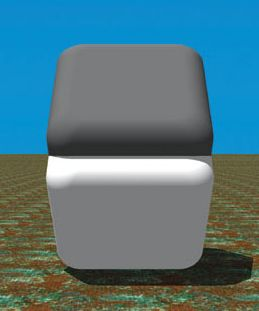
\includegraphics[height=.4\textheight]{figures/color-illusion.jpg}};
\node<3> at ([yshift=-1.5cm]current page.center) {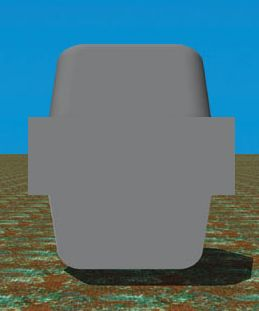
\includegraphics[height=.4\textheight]{figures/color-illusion2.jpg}};
\node<6> at ([yshift=-2.5cm]current page.center) {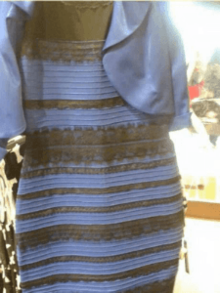
\includegraphics[height=.4\textheight]{figures/the-dress.png}};
\end{tikzpicture}


\end{frame}

\begin{frame}[c]\frametitle{Le daltonisme}

Environ un homme sur 10 est daltonien. 

\begin{center}
  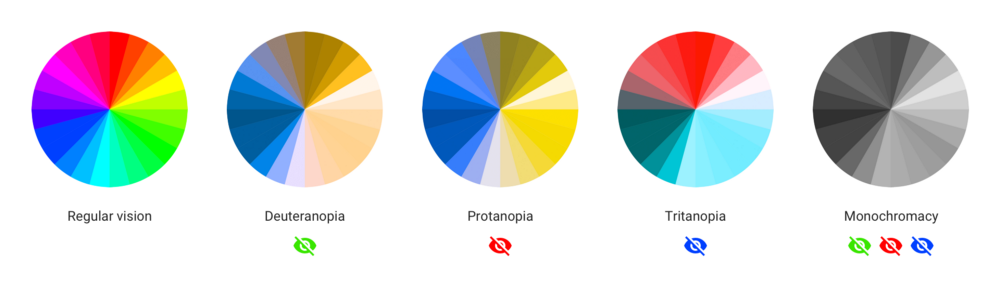
\includegraphics[width=1\textwidth]{figures/colorblindness-comparison.png}
\end{center}

\end{frame}






% \begin{frame}[c]\frametitle{Les palettes de couleurs}

% \vspace{-3mm}
% \RaggedRight\footnotesize
% \renewcommand{\arraystretch}{1.7}
% \begin{tabular}{lp{.27\textwidth}p{.27\textwidth}p{.27\textwidth}}
%  & \textbf{Qualitative} & \textbf{Séquentielle} & \textbf{Divergente}\\[1mm]
% Continues
% 	& \raisebox{-.35\height}{
\includegraphics[width=.25\textwidth]{palettes/qualitative_continuous.pdf}}
% 	& \raisebox{-.35\height}{
\includegraphics[width=.25\textwidth]{palettes/sequential_continuous.pdf}}
% 	& \raisebox{-.35\height}{
\includegraphics[width=.25\textwidth]{palettes/diverging_continuous.pdf}} \\
% Discrètes
% 	& \raisebox{-.35\height}{
\includegraphics[width=.25\textwidth]{palettes/qualitative_discrete.pdf}}
% 	& \raisebox{-.35\height}{
\includegraphics[width=.25\textwidth]{palettes/sequential_discrete.pdf}}
% 	& \raisebox{-.35\height}{
\includegraphics[width=.25\textwidth]{palettes/diverging_discrete.pdf}} \\
% Utilité & Catégories & Intensité & Déviation \\
% Propriétés 
% 	& 1 teinte par catégorie 
% 	& 1 teinte; le blanc marque le neutre
% 	& 2 teintes; le blanc marque le neutre\\
% Faiblesses 
% 	& Daltonisme, tons de gris
% 	& Difficile à analyser, affecté par les couleurs environnantes
% 	& Difficile à analyser, affecté par les couleurs environnantes \\
% Mitigations
% 	& Varier la luminosité, annoter
% 	& Échelle perceptuellement linéaire, annoter
% 	& Échelle perceptuellement linéaire, annoter
% \end{tabular}


% \end{frame}




\begin{frame}[c]\frametitle{Palettes qualitatives}

\vspace{1mm}

\begin{tabular}{@{}ll}
\RaggedRight\small
\renewcommand{\arraystretch}{2}
\begin{tabular}{@{}lp{.4\textwidth}}
\textbf{Utilité}
	& Catégories\\
\textbf{Propriétés}
	& 1 teinte par catégorie\\
\textbf{Faiblesses}
	& Daltonisme, tons de gris\\
\textbf{Mitigations}
	& Varier la luminosité, annoter\\
\end{tabular}
&
\begin{minipage}{.5\textwidth}
Continue
\vspace{1mm}


\includegraphics[width=.6\textwidth]{palettes/qualitative_continuous.pdf}

\vspace{2mm}

Discrète
\vspace{1mm}


\includegraphics[width=.6\textwidth]{palettes/qualitative_discrete.pdf}

\vspace{-2mm}
{
	\tiny
	\hspace{.32\textwidth}python2latex \textbf{holi}
}
\end{minipage} 
\end{tabular}

\pause
\vspace{4mm}
\small
\begin{tabular}{@{}p{.25\textwidth}@{}p{.25\textwidth}@{}p{.25\textwidth}@{}p{.25\textwidth}@{}}
Deuteranopia & Protanopia & Tritanopia & Monochromacy\\

\includegraphics[width=.2\textwidth]{palettes/qualitative-palette-deuteranopia.png} & 
\includegraphics[width=.2\textwidth]{palettes/qualitative-palette-protanopia.png} & 
\includegraphics[width=.2\textwidth]{palettes/qualitative-palette-tritanopia.png} & 
\includegraphics[width=.2\textwidth]{palettes/qualitative-palette-monochrome.png}\\
\end{tabular}


\end{frame}


% \begin{frame}[c]\frametitle{Palettes qualitatives}

% Se basent principalement sur les teintes (\textit{hue}) (ex. rouge, jaune, bleu...)

% Utiles pour différencier les catégories

% À proscrire pour les valeurs continues

% Une bonne palette qualitative\vspace{-\parskip}
% \begin{itemize}
% 	\item utilise des teintes \textit{perceptuellement} également espacées
% 	\item fait varier la luminosité des teintes
% \end{itemize}

% \end{frame}








\begin{frame}[c]\frametitle{Palettes séquentielles}

\vspace{0mm}

\begin{tabular}{@{}ll}
\RaggedRight\small
\renewcommand{\arraystretch}{1.7}
\begin{tabular}{@{}lp{.4\textwidth}}
\textbf{Utilité}
	& Intensité\\
\textbf{Propriétés}
	& 1 teinte; le pâle indique une faible intensité\\
\textbf{Faiblesses}
	& Difficile à analyser, affecté par les couleurs environnantes\\
\textbf{Mitigations}
	& Échelle perceptuellement linéaire, annoter\\
\end{tabular}
&
\begin{minipage}{.5\textwidth}
Continue
\vspace{1mm}


\includegraphics[width=.6\textwidth]{palettes/sequential_continuous.pdf}

\vspace{2mm}

Discrète
\vspace{1mm}


\includegraphics[width=.6\textwidth]{palettes/sequential_discrete.pdf}
\end{minipage} 
\end{tabular}

\pause
% \vspace{4mm}
\small
\textbf{Autres exemples}

\centering
\begin{tabular}{l@{\hskip10mm}l}
viridis & magma\\

\includegraphics[width=.3\textwidth]{palettes/sequential-viridis.png}
&

\includegraphics[width=.3\textwidth]{palettes/sequential-magma.png}
\end{tabular}


\end{frame}


% \begin{frame}[c]\frametitle{Palettes séquentielles}

% Se basent sur une ou deux teintes similaires et sur la luminosité

% Utiles pour représenter une intensité (avec un minimum/maximum de référence)

% Une bonne palette séquentielle\vspace{-\parskip}
% \begin{itemize}
% 	\item est \textit{perceptuellement} linéaire en teinte et luminosité
% 	\item est foncée pour les valeurs «~intenses~»
% \end{itemize}
% \end{frame}









\begin{frame}[c]\frametitle{Palettes divergentes}

\vspace{0mm}

\begin{tabular}{@{}ll}
\RaggedRight\small
\renewcommand{\arraystretch}{1.7}
\begin{tabular}{@{}lp{.4\textwidth}}
\textbf{Utilité}
	& Déviation\\
\textbf{Propriétés}
	& 2 teinte; le pâle indique le neutre\\
\textbf{Faiblesses}
	& Difficile à analyser, affecté par les couleurs environnantes\\
\textbf{Mitigations}
	& Échelle perceptuellement linéaire, annoter\\
\end{tabular}
&
\begin{minipage}{.5\textwidth}
Continue
\vspace{1mm}


\includegraphics[width=.6\textwidth]{palettes/diverging_continuous.pdf}

\vspace{2mm}

Discrète
\vspace{1mm}


\includegraphics[width=.6\textwidth]{palettes/diverging_discrete.pdf}
\end{minipage} 
\end{tabular}

\pause
% \vspace{4mm}
\centering
\small
\begin{tikzpicture}
\node(jet) {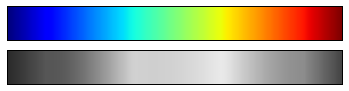
\includegraphics[width=.3\textwidth]{palettes/matplotlib-jet-palette.png}};
\node[anchor=south] at (jet.north) {matplotlib \textbf{jet}};

\draw[-, red, ultra thick] (jet.north east) -- (jet.south west);
\draw[-, red, ultra thick] (jet.south east) -- (jet.north west);

\node[anchor=west](turbo) at ([xshift=1cm]jet.east) {
\includegraphics[width=.3\textwidth]{palettes/diverging-turbo.png}};
\node[anchor=south] at (turbo.north) {Google \textbf{turbo}};


\draw (jet) -- (turbo);
\end{tikzpicture}


\end{frame}

% \begin{frame}[c]\frametitle{Palettes divergentes}
    
% Se basent sur deux teintes opposées et sur la luminosité

% Utiles pour représenter une déviation (avec une valeur «~centrale~» de référence)

% Une bonne palette divergente\vspace{-\parskip}
% \begin{itemize}
% 	\item est \textit{perceptuellement} linéaire en teinte et luminosité
% 	\item est saturée et foncée aux extrémités et lumineuse au centre
% 	\item utilise des teintes opposés (ex. bleu et orange, cyan et rouge)
% \end{itemize}
    
% \end{frame}



\begin{frame}[c]\frametitle{En résumé}

Moyen utile, mais plus ou moins fidèle.
Pour mitiger les faiblesses:\vspace{-\parskip}
\begin{itemize}
	\item Complémenter l'information (ex. annotations, formes)
	\item Palettes «~colorblind-safe~»
	\item \textbf{Luminosités} perceptuellement différentes
\end{itemize}

Outils:\vspace{-\parskip}
\begin{itemize}
	\item \href{https://colorbrewer2.org/}{\underline{ColorBrewer}} pour des palettes éprouvées
	\item \href{https://www.color-blindness.com/coblis-color-blindness-simulator/}{\underline{Coblis}}: Simulateur de daltonisme pour vérifier vos figures 
\end{itemize}

Références:\vspace{-\parskip}
\begin{itemize}
	\item \href{https://seaborn.pydata.org/tutorial/color_palettes.html}{\underline{seaborn}}
	\item \href{https://ai.googleblog.com/2019/08/turbo-improved-rainbow-colormap-for.html}{\underline{Google turbo}}
\end{itemize}

\end{frame}




\begin{frame}

\centering \bf
\Huge \color{couleurTheme} Bonne session!

\end{frame}




\end{document}